%%%%%%%%%%%%%%%%%%%%%%%%%%%%%%%%%%%%%%%%%%%%%%%%%%%%%%%%%%%%%%%%%%%%%%%%%%%%%%%%
%2345678901234567890123456789012345678901234567890123456789012345678901234567890
%        1         2         3         4         5         6         7         8

\documentclass[letterpaper, 10 pt, conference]{ieeeconf}  % Comment this line 
%                                                         % out if you need a4
%\documentclass[a4paper, 10pt, conference]{ieeeconf}      % Use this line for a4
                                                          % paper

% \IEEEoverridecommandlockouts                            % This command is only
%                                                         % needed if you want 
%                                                         % to use the \thanks 
%                                                         % command
\overrideIEEEmargins
% See the \addtolength command later in the file to balance the column lengths
% on the last page of the document



% The following packages can be found on http:\\www.ctan.org
\usepackage{graphicx} % for pdf, bitmapped graphics files\
\usepackage{subcaption}
\usepackage{amsmath}
\usepackage{booktabs}
\usepackage{hyperref}

\title{\LARGE \bf
Hing-King-Linden Score: 
A robust method of assessing foosball matchups independent of tournament 
structure
}

\author{Philip Linden, Adam King and Brandon Hing% <-this % stops a space
}

\begin{document}

\maketitle
\thispagestyle{empty}
\pagestyle{empty}


%%%%%%%%%%%%%%%%%%%%%%%%%%%%%%%%%%%%%%%%%%%%%%%%%%%%%%%%%%%%%%%%%%%%%%%%%%%%%%%%
\begin{abstract}

The results of randomly seeded single-elimination tournaments does not reflect a
player or team's relative rank, or foosball performance score. Existing ranking
such as Elo Ranking or Swiss systems depend on a large number of matches to be
played to produce accurate results. We present a method of determining rank
using the relative performance of a player's opponent and the points scored on
that opponent during a foosball match. We demonstrate that the Hing-King-Linden
Score, or HKL, is a robust method of predicting foosball matchups between two
players or teams, and a reliable way to seed teams and tournaments fairly based
on only the number of matches played and tracking points scored against each
opponent. We show the utility of HKL using the real results of a randomly seeded
single-elimination tournament.

\end{abstract}


%%%%%%%%%%%%%%%%%%%%%%%%%%%%%%%%%%%%%%%%%%%%%%%%%%%%%%%%%%%%%%%%%%%%%%%%%%%%%%%%
\section{INTRODUCTION}

Championship tournaments are a tried-and-true organization for competitions in
sports today, and foosball is no exception. However, both single- and
double-elimination tournament results are predicated upon fair seeding of the
matchups at the start of the tournament. Some existing ranking systems used to
seed tournaments are Elo Ranking \cite{elo}, used for the FIFA World Cup
\cite{fifa}, or the Swiss-system \cite{swiss}, commonly used in chess
tournaments \cite{chess}. A fair score in both Elo and Swiss systems requires
that each member of the tournament plays every other in round-robin fashion,
where $\frac{n}{2}(n-1)$ matches must be played before a rank is determined. The
difference in these rankings is in how scores incorporate margin of victory and
win/loss rates. Additionally, existing rating systems assume that results are
binary (win or loss) or uncapped scores (higher score wins). In foosball, wins
are determined by the first team to score a set number of points. 

In a recent tournament, the competition organizers used a single-elimination
tournament between 16 randomly seeded players to seed an 8-team tournament of
evenly matched 2-person teams. In this event structure, we must determine
relative skill of 16 players when the conditions for Elo and Swiss rankings
systems are not met---not only have players not played at least one match
against one another, but some players played more matches than others. In some
cases, players eliminated in the first round scored more points and lost by a
smaller margin of victory against the overall winner of the tournament. Thus it
is clear that a robust ranking system is needed to assemble fair teams based on
match results using the relative performance of a player's opponent to determine
that player's rank.

In this paper we propose the Hing-King-Linden Score, or HKL, which weighs the
cumulative number of points scored against each opponent and the relative
performance of that opponent. Critically, HKL only requires one randomly seeded
single-elimination tournament to determine an accurate score that reflects
relative performance. 

The primary goal of the HKL is to rank contestants fairly given the following
principles:

\begin{enumerate}
        \item Given two players who lose a match in the same round of the
        tournament by the same margin of victory, the player whose opponent
        progresses through more subsequent rounds should have a higher HKL.
        \item The winner of a randomly-seeded single-elimination tournament does
        not necessarily have the highest rank.
        \item Two players with similar HKL compete with similar performance.
\end{enumerate}

\section{DEFINITION}
As matches are played, points scored are tracked individually for each player
per opponent. Points scored per opponent are cumulative, but in a
single-elimination tournament no pair of contestants appears in the bracket more
than once.

\begin{figure}[hb]
        \includegraphics[width=\linewidth]{fig/score-matrix.png}
        \label{fig:raw-score}
        \centering
        \caption{Points scored are tracked per opponent for each player.}
\end{figure}

Since some players progress further than others in the bracket and thus have
more scoring opportunities in every round, it is necessary to normalize the
total points scored per opponent, $p$, by a player's progression in the
tournament, $r$, where $r$ is the number of matches that a player has completed.


\begin{equation}
        \hat{p} = p/r
        \label{eq:normalized-score}
\end{equation}

\begin{figure}[ht]
        \includegraphics[width=\linewidth]{fig/normalized-score-matrix.png}
        \label{fig:normalized-score}
        \centering
        \caption{Scored points are normalized by progression in the tournament.}
\end{figure}

A player's overall performance, $k$, is then calculated as the root-sum-square
of the normalized total points scored and progression in the tournament. By
using the root-sum-square of progression and normalized scores, we estimate how
consistently a player performs in the tournament. A high performing player is
likely to win many rounds of the tournament by large margins while a weaker
player might win some matches but by small margins. Conversely, a player that
scores many points in just a few matches is more likely to be a strong player.

\begin{equation}
        k = \sqrt{\hat{p}^2 + r^2}
        \label{eq:skill-indicator}
\end{equation}

To provide a basis for comparison between player performance scores, we linearly
scale $k$ to an arbitrary fixed range, such as $n = (0,10)$, to compose a
player's Power Rating, $H$. Since this scale is relative, scaling depends on the
maximum and minumum $k$ in the set of all players in the tournament.

\begin{equation}
        K = n_1 + \left(\frac{n_2 - n_1}{\text{max}(k) - \text{min}(k)}\right)(k - \text{min}(k))  
        \label{eq:power-rating}
\end{equation}

Since $k$ is independent of a player's opponent, we can estimate the relative
difficulty of any matchup between two players, $d$, with a simple ratio. A
difficulty of $d<1$ indicates an ``easy'' match while $d>1$ indicates a
``difficult'' match from the perspective of any player against any opponent. A
perfectly even matchup results in $d=1$, which makes sense if considering the
most perfect matchup---a player versus themselves---is unity difficulty. For
reporting, we may scale difficulty using \autoref{eq:power-rating}, replacing
$k$ with $d$. 

\begin{equation}
        d = \frac{k_{player}}{k_{opponent}}
        \label{eq:matchup-difficulty}
\end{equation}

\begin{figure}[ht]
        \includegraphics[width=\linewidth]{fig/matchup-difficulty-matrix.png}
        \label{fig:matchup-difficulty}
        \centering
        \caption{The ratio of $d$ for any matchup indicates the relative 
                 difficulty for one player against another.}
\end{figure}

Next, we weigh the number of points scored per opponent by the matchup
difficulty against that opponent. In other words, a point scored in a difficult
match is ``worth'' more than a point scored in an easy match, regardless of
which round of the tournament the point was scored. We estimate a player's
cumulative performance, $s$, by summing the total adjusted points, $\bar{p}$,
scored in all rounds of the tournament. Again, we linearly scale $s$ to
arbitrary range $n$ to ground it in a relative basis, and map it to the same
scale as $K$. The scaled performance metric, $S$, is called a player's Seed
Rating.

\begin{equation}
        \bar{p} = p d
        \label{eq:adjusted-score}
\end{equation}

\begin{equation}
        s = \sum{\bar{p}}
        \label{eq:unscaled-seed-rating}
\end{equation}

\begin{equation}
        S = n_1 + \left(\frac{n_2 - n_1}{\text{max}(s) - \text{min}(s)}\right)
        (s - \text{min}(s))  
        \label{eq:seed-rating}
\end{equation}

Finally, we assert that Power Rating, $K$, and Seed Rating, $S$, are equally
justified as indicators of a player's performance. We see that Power Rating
estimates performance over many matches while Seed Rating accounts for
performance in individual matches. Thus we arrive at the HKL, $H$, defined as
the average between the Power and Seed Ratings. Since $K$ and $S$ are scaled to
the same fixed range, $H$ is also scaled to that range.

\begin{equation}
        H = (K + S)/2
        \label{eq:hkl-score}
\end{equation}

\begin{table}[hb]
        \begin{tabular}{lccc|ccc}
                \toprule
                &\multicolumn{3}{c}{Parameters} & \multicolumn{3}{c}{Rankings}\\
                \midrule
                Player  & $r$   & $\hat{p}$ & $k$ & $S$ & $K$   & $H$ \\
                \midrule
                Abhra	& 1	& 0.00	& 1.00	& 0.00	& 0.00	& 0.00 \\
                Adam	& 1	& 4.00	& 4.12	& 2.45	& 5.78	& 4.11 \\
                Ben	& 3	& 4.33	& 5.27	& 5.66	& 7.90	& 6.78 \\
                Bethany	& 1	& 4.00	& 4.12	& 4.35	& 5.78	& 5.06 \\
                Brandon	& 2	& 3.00	& 3.61	& 4.09	& 4.82	& 4.46 \\
                Caleb	& 4	& 5.00	& 6.40	& 10.00	& 10.00	& 10.00 \\
                Cruz	& 4	& 4.25	& 5.84	& 7.96	& 8.95	& 8.45 \\
                Jeff	& 1	& 2.00	& 2.24	& 2.52	& 2.29	& 2.41 \\
                Kyle	& 1	& 1.00	& 1.41	& 2.89	& 0.77	& 1.83 \\
                Lisa	& 1	& 4.00	& 4.12	& 2.74	& 5.78	& 4.26 \\
                Matt	& 2	& 3.50	& 4.03	& 5.60	& 5.61	& 5.61 \\
                Natasha	& 2	& 3.50	& 4.03	& 3.59	& 5.61	& 4.60 \\
                Phil	& 1	& 3.00	& 3.16	& 2.39	& 4.00	& 3.20 \\
                Sean	& 2	& 3.00	& 3.61	& 5.24	& 4.82	& 5.03 \\
                Steve	& 1	& 1.00	& 1.41	& 2.61	& 0.77	& 1.69 \\
                Tyler	& 3	& 3.67	& 4.74	& 4.66	& 6.92	& 5.79 \\
                \bottomrule
        \end{tabular}
        \centering
        \caption{Example HKL and intermediate parameters}
        \label{tab:example-ratings}
\end{table}

\section{FEATURES}
Since HKL is relative between all members of a tournament and only depends on 
scores earned during matches, four major advantages emerge from this new ranking
method:

\begin{enumerate}
        \item HKL of all contestants is defined as soon as one match is
        completed by every contestant.
        \item HKL can be updated during a match that has not yet completed.
        \item HKL is independent of which matches on the tournament schedule are
        played, and independent of the order that they are played.
        \item HKL remains valid for comparisons between contestants who have
        played a different number of matches.
\end{enumerate}

Another feature of the HKL that it is purely additive in nature. Even if a
strong player loses a match to a opponent with a much lower rank, the stronger
player still earns points. In other words, all parameters are greater than or
equal to zero. This means that the only way a player's HKL can decrease is if
the minimum or maximum of the sets of all $k$ or all $s$ change. 

\subsection{Example Scenario: No decrease in HKL after a match}
Two players, $A$ and $B$, play a match with a matchup diffulty $d=1$. At the
start of the match, their performance parameters, $k$ and $s$, are greater than
the performance parameters of player $C$, but less than the performance
parameters of player $D$, who has the highest HKL out of all players in the
tournament. The final score is $5-0$ and player $A$ wins the match. The number
of matches completed, $r$, for both players increases by $1$. Even though player
$B$ did not score any points, it is not possible for their $k$ or $s$ to
decrease, and the performance parameters of both players is still higher than
player $C$. Player $A$ has scored enough adjusted points, $\bar{p}$, to tie
player $D$ in $s$ but has played more matches than player $D$ and still has a
lower $k$ score. In this example, the minimum and maximum $s$ and $k$ out of all
players in the tournament has not changed. Therefore both player $A$ and player
$B$ gain in Seed Rating, $S$, and Power Rating, $K$, but no other players in the
tournament see a decrease in HKL.

% \subsection{Example Scenario: Applying HKL in a double elimination tournament}
% Since HKL is evaluated using scores normalized by the number of matches played
% (\autoref{eq:normalized-score}), no adjustments to the HKL calculations are
% required to compare the performance of players in the primary bracket and the
% consolation bracket of a double elimination tournament. For example, consider
% player $A$ and player $B$, where player $A$ loses to player $B$ in the first
% round of the primary bracket then wins all matches in the consolation bracket,
% and player $B$ wins all matches in the primary bracket. The structure of a
% double elimination bracket now leads to a rematch between $A$ and $B$ for the
% championship, but player $A$ has necessarily played one more game than player
% $B$ thus far. Since we normalize the accrued points by the number of games
% played, we can directly compare the HKL between $A$ and $B$.

% \subsection{Example Scenario: Predicting a winner in a ``perfect'' matchup}
% $k$ predicts long term trends (finishing matches) but $s$ accounts for per-game
% (transient, dynamic) performance

% \section{CONCLUSION}

%%%%%%%%%%%%%%%%%%%%%%%%%%%%%%%%%%%%%%%%%%%%%%%%%%%%%%%%%%%%%%%%%%%%%%%%%%%%%%%%
\section*{ACKNOWLEDGMENTS}
The authors thank Tyler Brown and Hamil Sulaiman for their continued support
toward foosball matches and the application of the statistics they create.

%%%%%%%%%%%%%%%%%%%%%%%%%%%%%%%%%%%%%%%%%%%%%%%%%%%%%%%%%%%%%%%%%%%%%%%%%%%%%%%%

\bibliography{hkl-score.bib}
\bibliographystyle{IEEEtran}

%%%%%%%%%%%%%%%%%%%%%%%%%%%%%%%%%%%%%%%%%%%%%%%%%%%%%%%%%%%%%%%%%%%%%%%%%%%%%%%%
\onecolumn
\section*{APPENDIX}
\setcounter{section}{0}

\section{CASE STUDY: PREDICTION ACCURACY OVER A SINGLE-ELINIMATION TOURNAMENT}
% Show how HKL changes with predictions as a tournament is played
Like other ranking systems, HKL accuracy increases with the number of matches
played. In this section, we demonstrate how HKL predicts match results and how
these predictions respond to match results using real data collected during a
single elimination tournament.

% \subsection{Tournament Format}
% Show bracket and player score matrix

\subsection{Asynchronous tournament progression}
\begin{figure}[h!b]
        \centering
        \begin{subfigure}[ht]{0.5\textwidth}
                \centering
                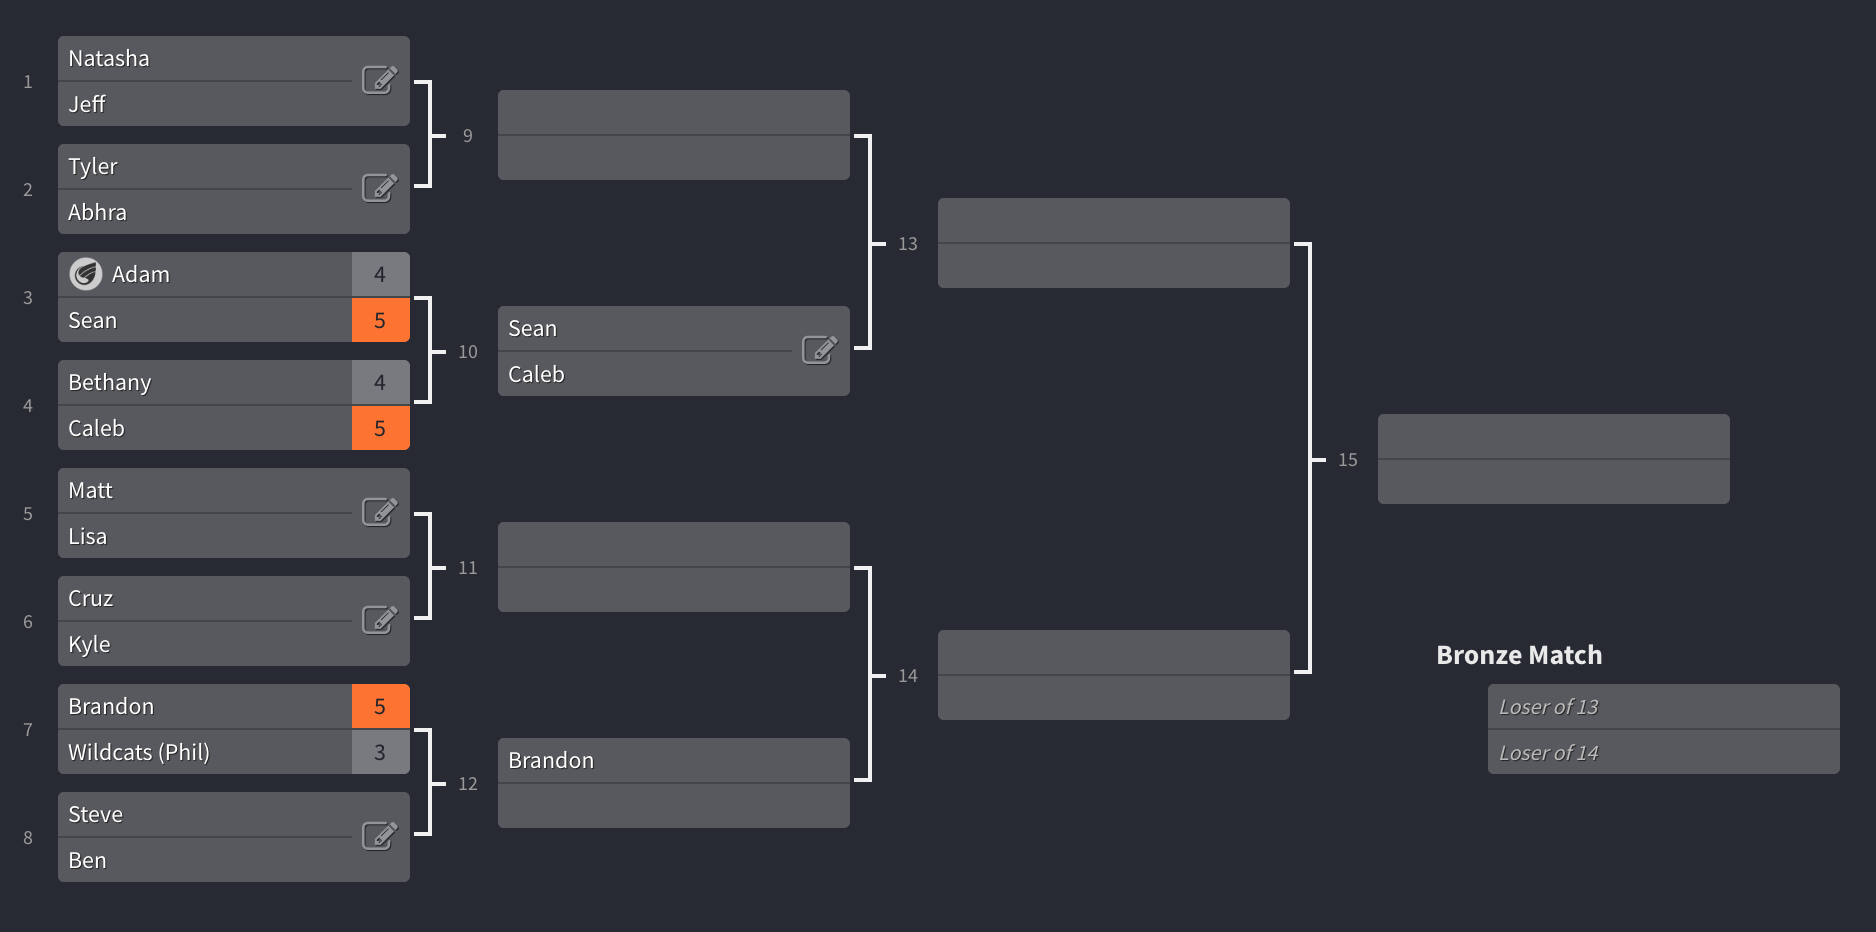
\includegraphics[width=0.9\textwidth]{fig/singles-bracket_1.png}
                \caption{Tournament bracket}
        \end{subfigure}
        \begin{subfigure}[ht]{0.4\textwidth}
                \centering
                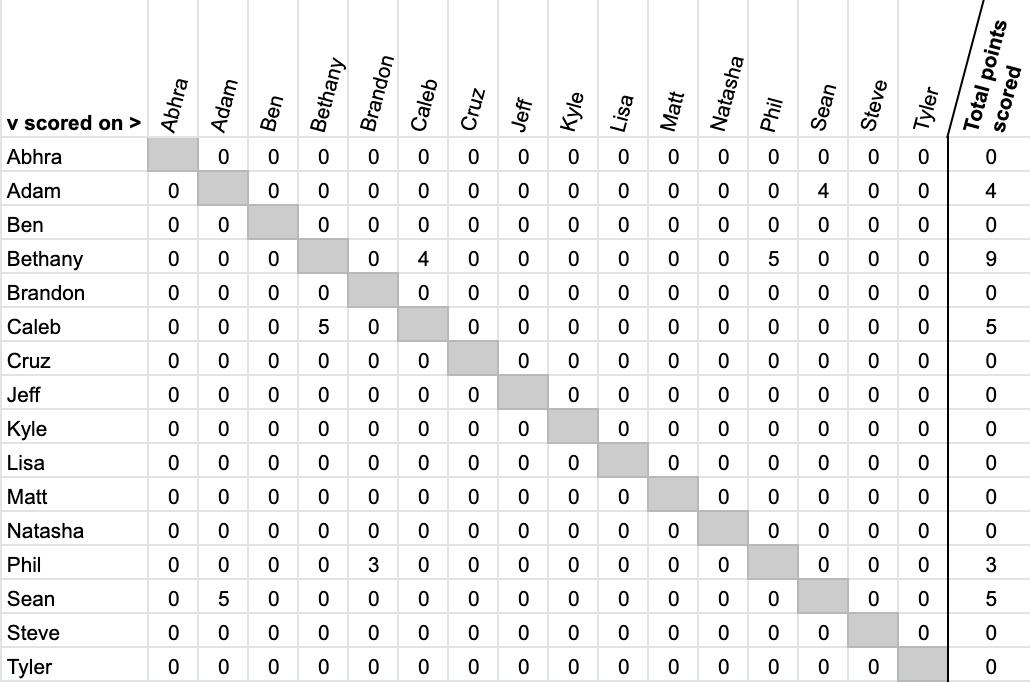
\includegraphics[width=0.9\textwidth]{fig/score-matrix_1.png}
                \caption{Score matrix}
        \end{subfigure}

        \begin{subfigure}[hb]{0.5\textwidth}
        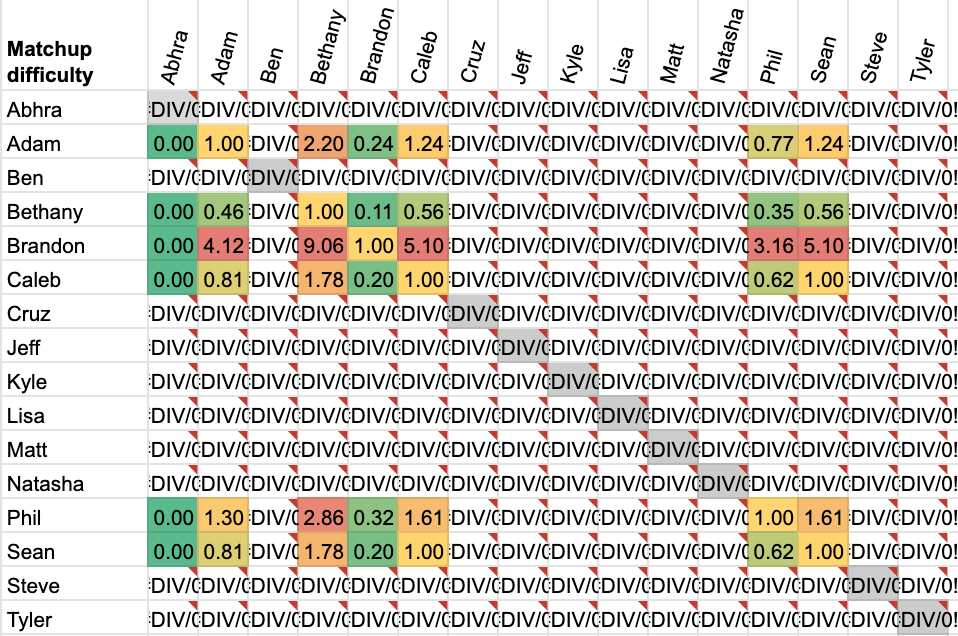
\includegraphics[width=0.9\textwidth]{fig/difficulty_1.png}
        \caption{Match difficulty predictor, $d$.}
        \end{subfigure}
        \begin{subfigure}[hb]{0.4\textwidth}
                \footnotesize
                \centering
                \begin{tabular}{lccc|ccc}
                        \toprule
                        Player  & $r$   & $\hat{p}$ & $k$ & $S$ & $K$ & $H$\\
                        \midrule
                        Abhra	& 0	& 0.00	& 0.00 & - & - & - \\
                        Adam	& 1	& 4.00	& 4.12 & - & - & - \\
                        Ben	& 0	& -	& -    & - & - & - \\
                        Bethany	& 1	& 4.00	& 4.12 & - & - & - \\
                        Brandon	& 1	& 3.00	& 3.61 & - & - & - \\
                        Caleb	& 1	& 5.00	& 6.40 & - & - & - \\
                        Cruz	& 0	& 4.25	& 5.84 & - & - & - \\
                        Jeff	& 0	& -	& -    & - & - & - \\
                        Kyle	& 0	& -  	& -    & - & - & - \\
                        Lisa	& 0	& -  	& -    & - & - & - \\
                        Matt	& 0	& -  	& -    & - & - & - \\
                        Natasha	& 0	& -  	& -    & - & - & - \\
                        Phil	& 1	& 3.00	& 3.16 & - & - & - \\
                        Sean	& 1	& 3.00	& 3.61 & - & - & - \\
                        Steve	& 0	& -  	& -    & - & - & - \\
                        Tyler	& 0	& -  	& -    & - & - & - \\
                        \bottomrule
                \end{tabular}
                \caption{Player scores.}
        \end{subfigure}
        \caption{Match difficulty can be predicted for matchups between 
                 any player who has completed one game.}
\end{figure}

\begin{figure}[h!b]
        \centering
        \begin{subfigure}[ht]{0.5\textwidth}
                \centering
                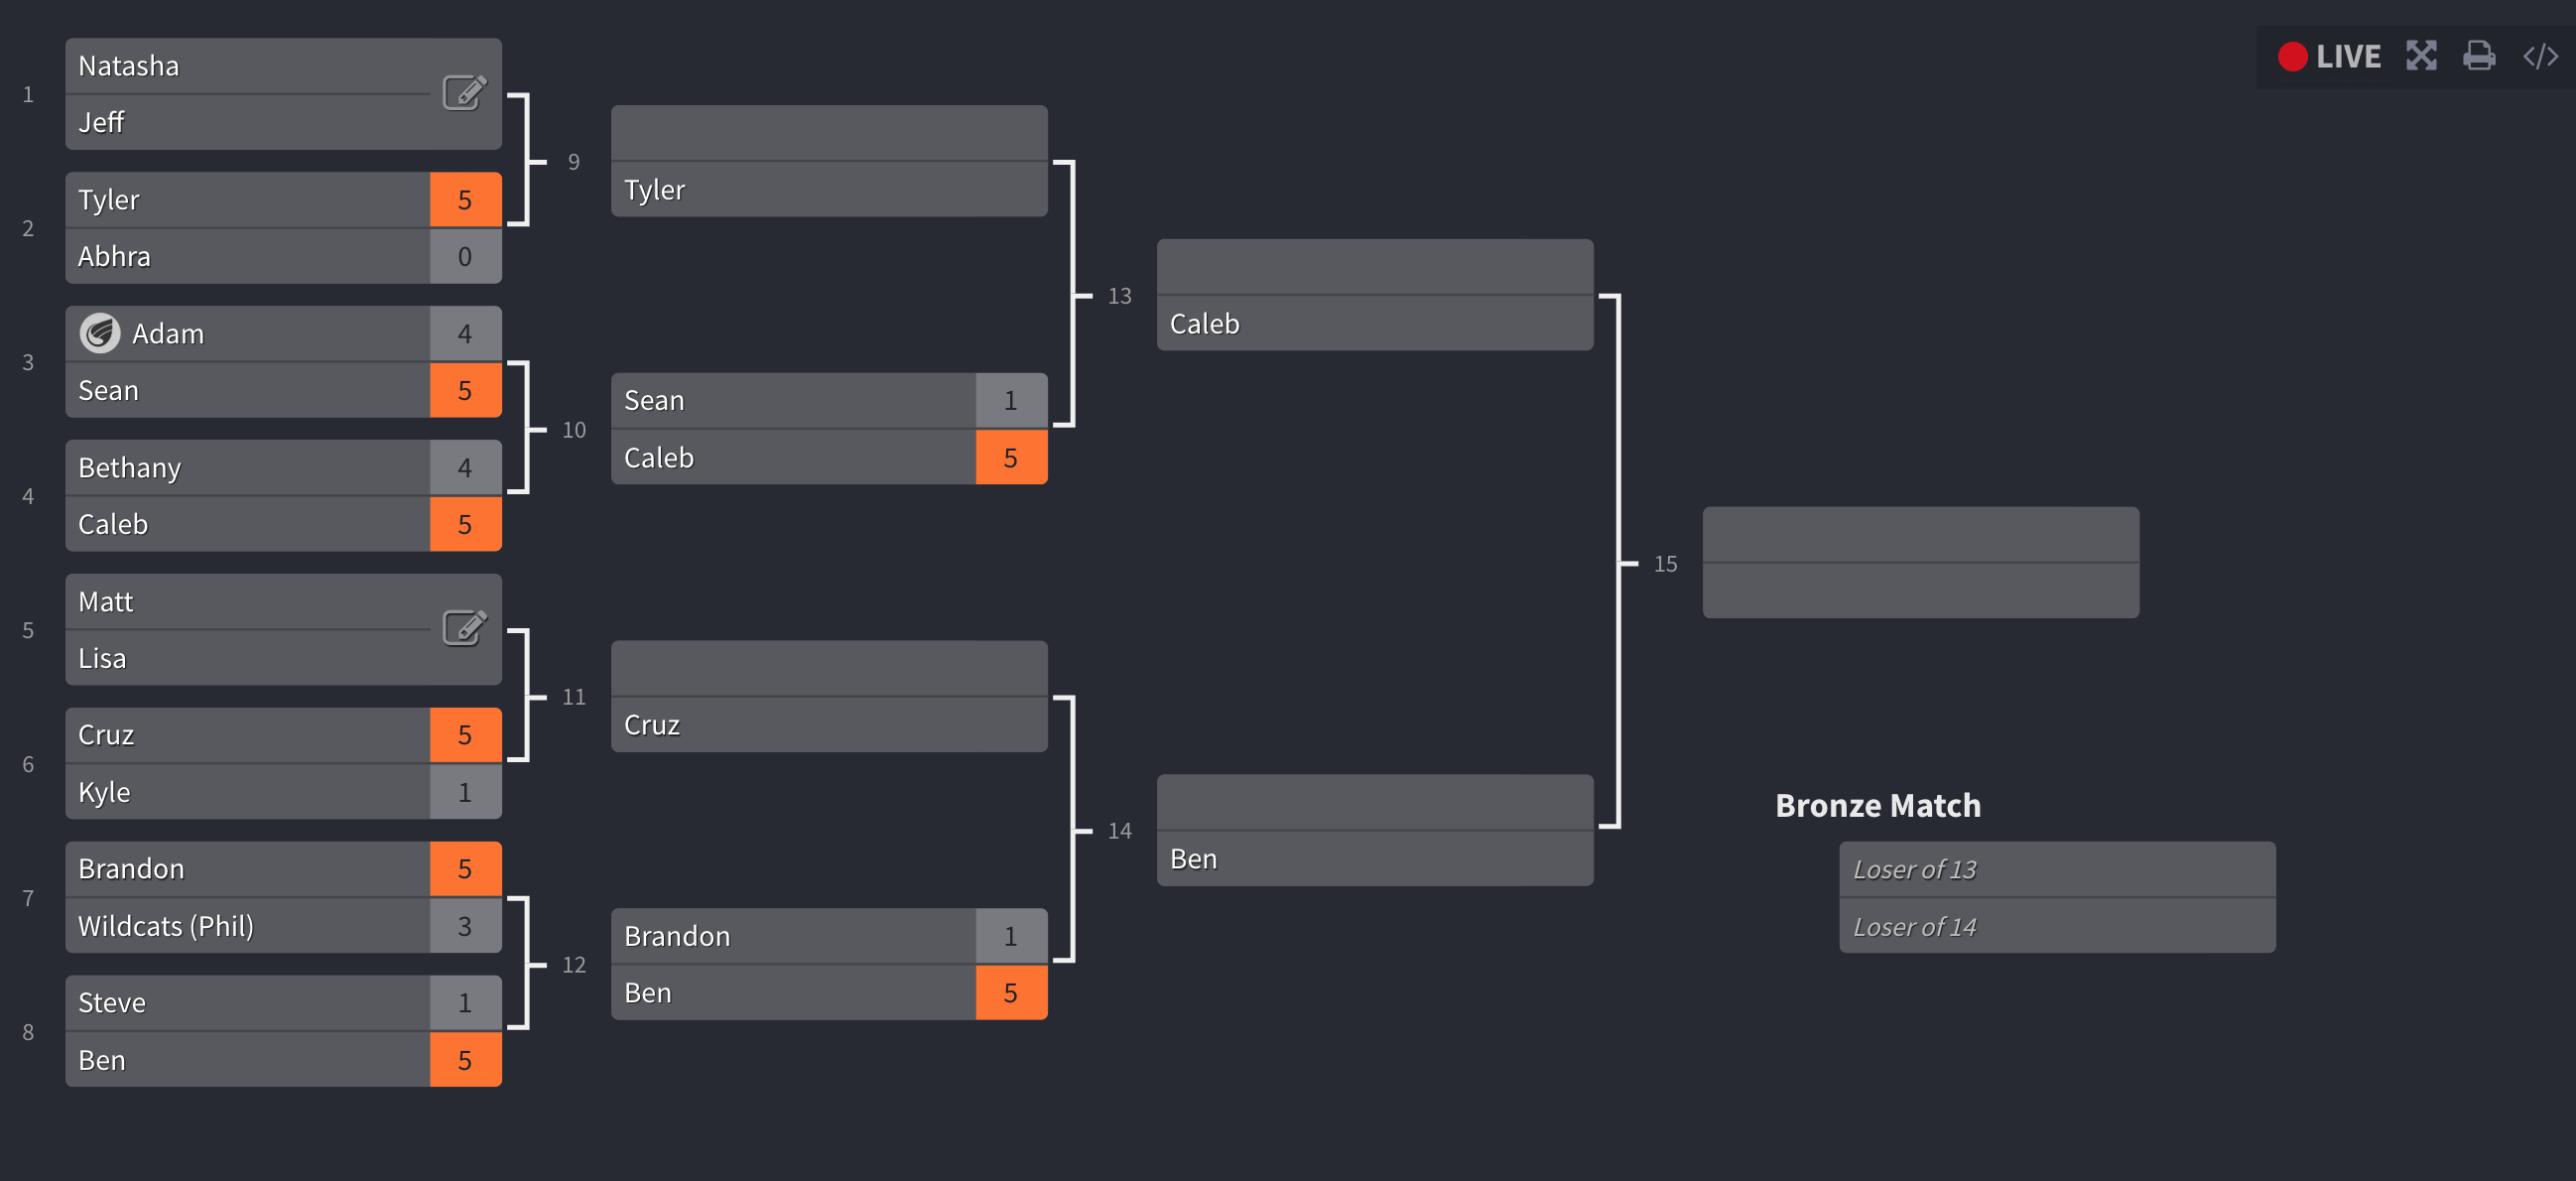
\includegraphics[width=0.9\textwidth]{fig/singles-bracket_3.png}
        \end{subfigure}
        \begin{subfigure}[ht]{0.4\textwidth}
                \centering
                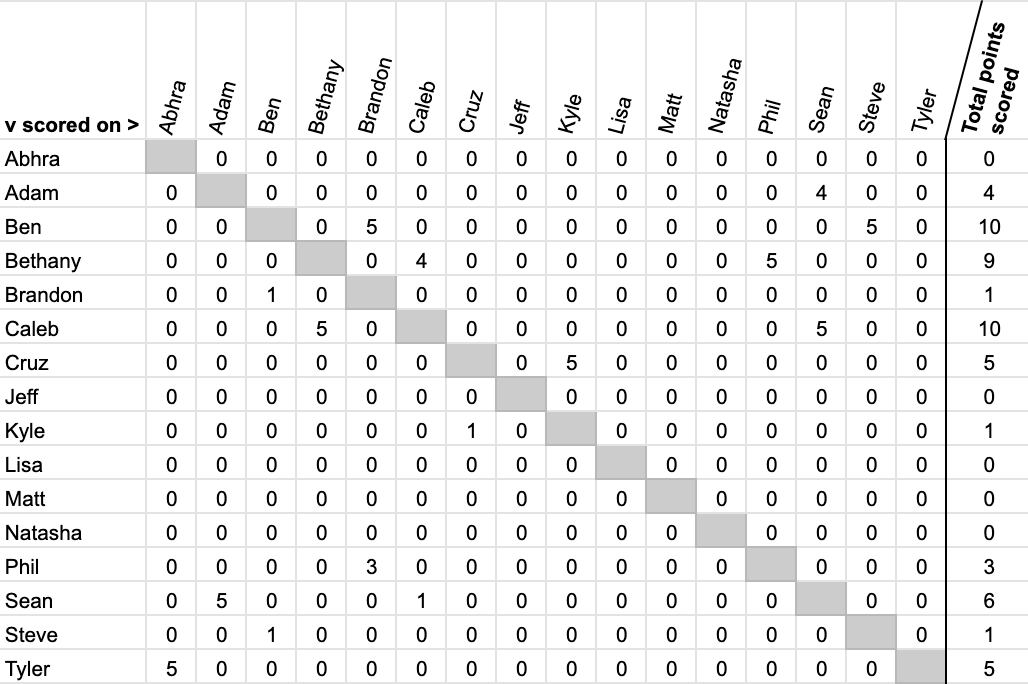
\includegraphics[width=0.9\textwidth]{fig/score-matrix_3.png}
        \end{subfigure}
        \begin{subfigure}[hb]{0.5\textwidth}
                \centering
                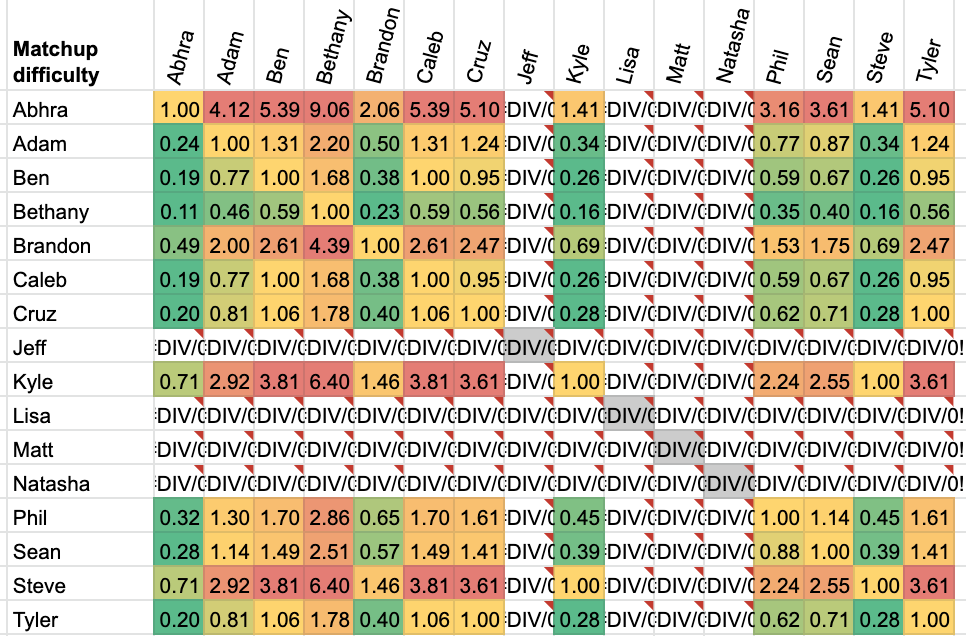
\includegraphics[width=0.9\textwidth]{fig/difficulty_3.png}
        \end{subfigure}
        \begin{subfigure}[hb]{0.4\textwidth}
                \footnotesize
                \centering
                \begin{tabular}{lccc|ccc}
                        \toprule
                        Player  & $r$   & $\hat{p}$ & $k$ & $S$ & $K$ & $H$ \\
                        \midrule
                        Abhra	& 1	& 0.00	& 0.00 & - & - & - \\
                        Adam	& 1	& 4.00	& 4.12 & - & - & - \\
                        Ben	& 2	& 5.00	& 5.39 & - & - & - \\
                        Bethany	& 1	& 9.00	& 9.06 & - & - & - \\
                        Brandon	& 2	& 0.50	& 2.06 & - & - & - \\
                        Caleb	& 2	& 5.00	& 5.39 & - & - & - \\
                        Cruz	& 1	& 5.00	& 5.10 & - & - & - \\
                        Jeff	& 0	& -  	& -    & - & - & - \\
                        Kyle	& 1	& 1.00	& 1.41 & - & - & - \\
                        Lisa	& 0	& -  	& -    & - & - & - \\
                        Matt	& 0	& -  	& -    & - & - & - \\
                        Natasha	& 0	& -  	& -    & - & - & - \\
                        Phil	& 1	& 3.00	& 3.16 & - & - & - \\
                        Sean	& 2	& 3.00	& 3.61 & - & - & - \\
                        Steve	& 1	& 1.00 	& 1.41 & - & - & - \\
                        Tyler	& 1	& 5.00  & 5.10 & - & - & - \\
                        \bottomrule
                \end{tabular}
        \end{subfigure}
        \caption{Since player performance is scaled by the number of matches
                 played, valid predictions can be made about matchups between
                 any player who has completed at least one game. HKL requires
                 all players in the tournament to play one game before can be
                 determined.}
\end{figure}

\begin{figure}[h!b]
        \centering
        \begin{subfigure}[ht]{0.5\textwidth}
                \centering
                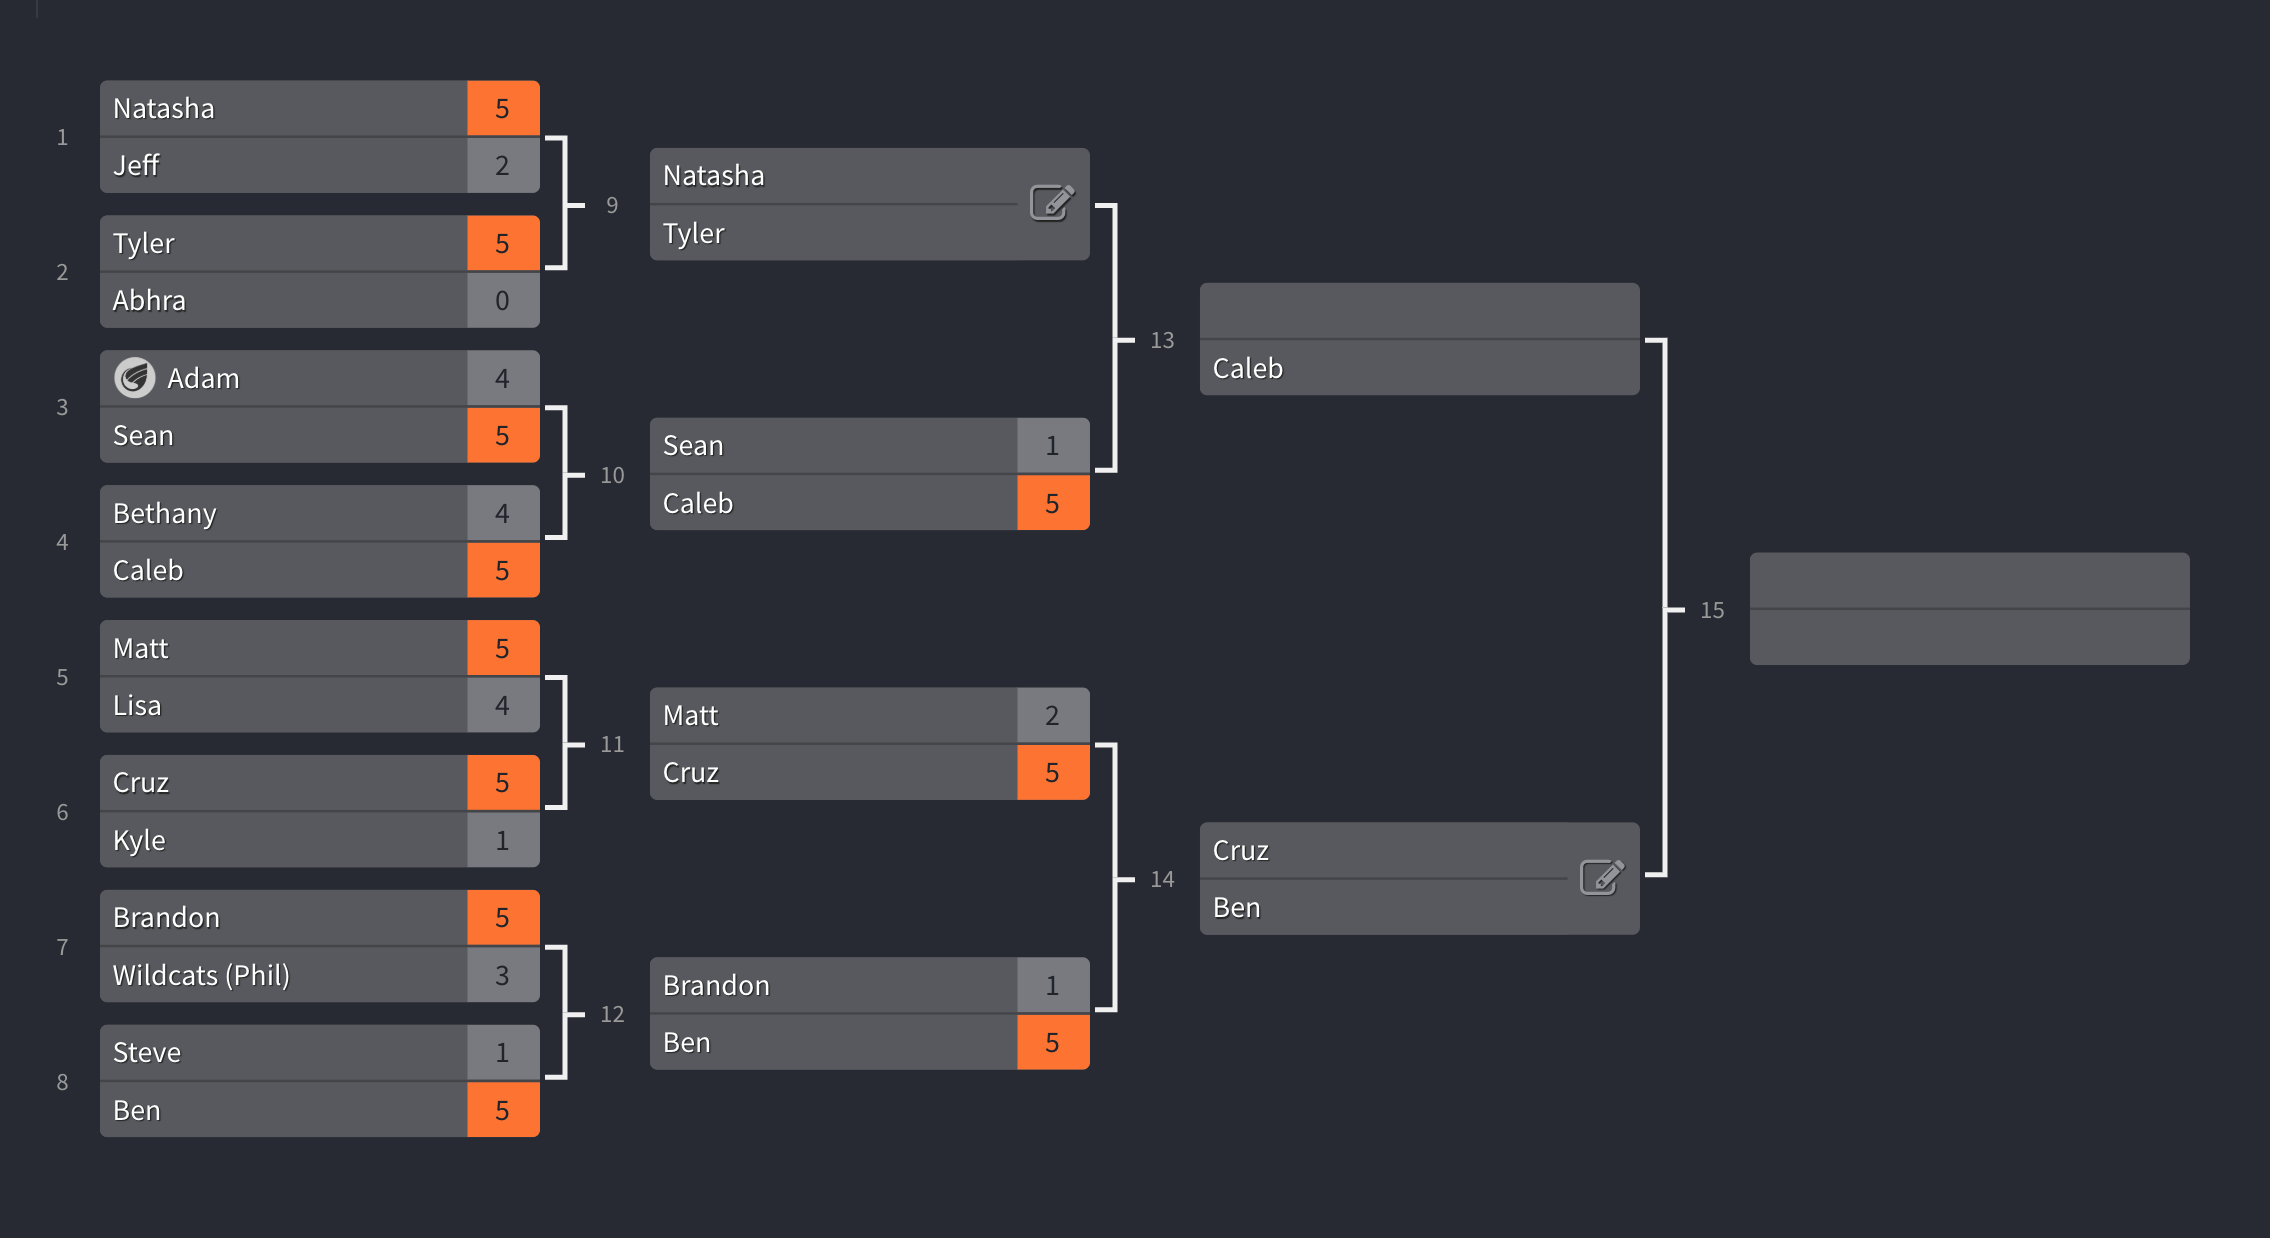
\includegraphics[width=0.9\textwidth]{fig/singles-bracket_4.png}
        \end{subfigure}
        \begin{subfigure}[ht]{0.4\textwidth}
                \centering
                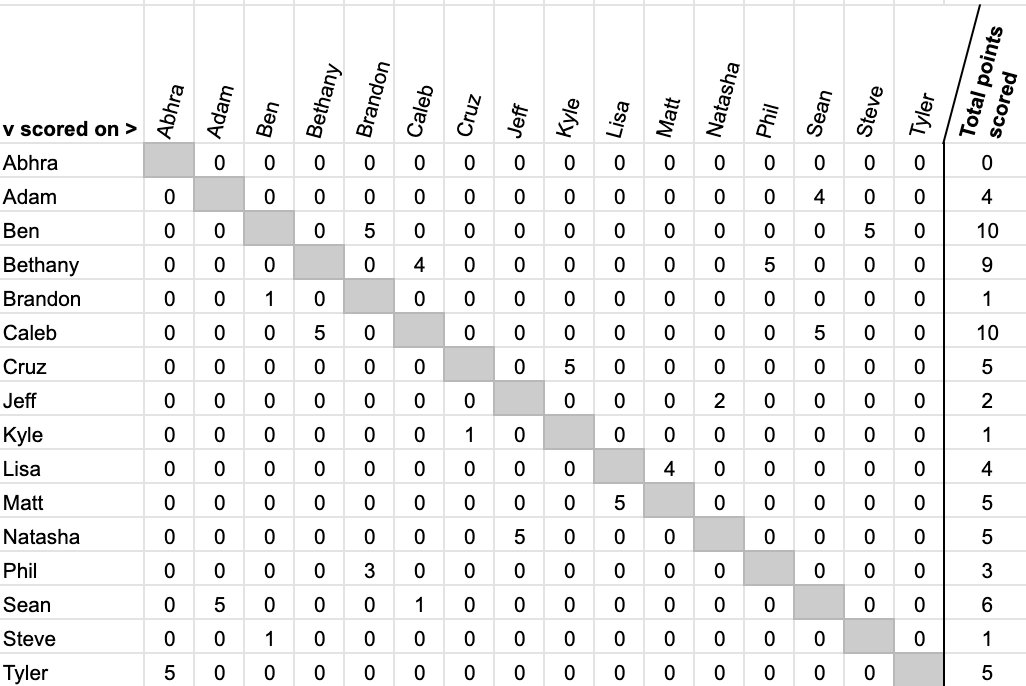
\includegraphics[width=0.9\textwidth]{fig/score-matrix_4.png}
        \end{subfigure}
        
        \begin{subfigure}[hb]{0.5\textwidth}
                \centering
                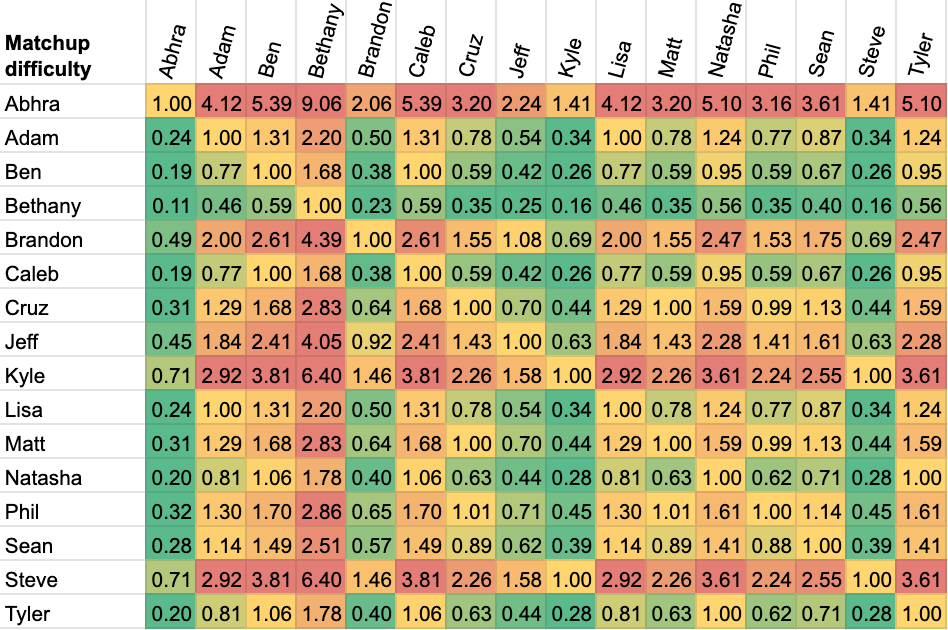
\includegraphics[width=0.9\textwidth]{fig/difficulty_4.png}
        \end{subfigure}
        \begin{subfigure}[hb]{0.4\textwidth}
                \footnotesize
                \centering
                \begin{tabular}{lccc|ccc}
                        \toprule
                        Player  & $r$   & $\hat{p}$ & $k$ & $S$ & $K$ & $H$ \\
                        \midrule
                        Abhra	& 1	& 0.00	& 0.00 & 0.00 & 0.00 & 0.00 \\
                        Adam	& 1	& 4.00	& 4.12 & 2.98 & 3.88 & 3.43 \\
                        Ben	& 2	& 5.00	& 5.39 & 2.75 & 5.44 & 4.09 \\
                        Bethany	& 1	& 9.00	& 9.06 & 3.51 & 10.00 & 6.75 \\
                        Brandon	& 2	& 0.50	& 2.06 & 2.22 & 1.32 & 1.77 \\
                        Caleb	& 2	& 5.00	& 5.39 & 10.00 & 5.44 & 7.72 \\
                        Cruz	& 2	& 2.50	& 3.20 & 1.88 & 2.73 & 2.31 \\
                        Jeff	& 1	& 2.00  & 2.24 & 3.88 & 1.53 & 2.71 \\
                        Kyle	& 1	& 1.22	& 1.41 & 1.93 & 0.51 & 1.22 \\
                        Lisa	& 1	& 4.00  & 4.12 & 2.94 & 3.88 & 3.26 \\
                        Matt	& 2	& 2.50  & 3.20 & 5.48 & 2.73 & 4.11 \\
                        Natasha	& 1	& 5.00  & 5.10 & 1.87 & 5.09 & 3.48 \\
                        Phil	& 1	& 3.00	& 3.16 & 1.66 & 2.68 & 2.17 \\
                        Sean	& 2	& 3.00	& 3.61 & 6.13 & 3.23 & 4.68 \\
                        Steve	& 1	& 1.00 	& 1.41 & 3.24 & 0.51 & 1.88 \\
                        Tyler	& 1	& 5.00  & 5.10 & 0.83 & 5.09 & 2.96 \\
                        \bottomrule
                \end{tabular}
        \end{subfigure}
        \caption{Once every player has completed at least one match, HKL for all 
                 players is determined.}
\end{figure}
\clearpage

\subsection{Reacting to upsets}

\begin{figure}[h!b]
        \centering
        \begin{subfigure}[hb]{0.4\textwidth}
                \footnotesize
                \centering
                \begin{tabular}{lccc|ccc}
                        \toprule
                        Player  & $r$   & $\hat{p}$ & $k$ & $S$ & $K$ & $H$ \\
                        \midrule
                        Abhra	& 1	& 0.00	& 0.00 & 0.00 & 0.00 & 0.00 \\
                        Adam	& 1	& 4.00	& 4.12 & 2.98 & 3.88 & 3.43 \\
                        \textbf{Ben}	& \textbf{2}	& \textbf{5.00}	& \textbf{5.39} & \textbf{2.75} & \textbf{5.44} & \textbf{4.09} \\
                        Bethany	& 1	& 9.00	& 9.06 & 3.51 & 10.00 & 6.75 \\
                        Brandon	& 2	& 0.50	& 2.06 & 2.22 & 1.32 & 1.77 \\
                        Caleb	& 2	& 5.00	& 5.39 & 10.00 & 5.44 & 7.72 \\
                        \textbf{Cruz}	& \textbf{2}	& \textbf{2.50}	& \textbf{3.20} & \textbf{1.88} & \textbf{2.73} & \textbf{2.31} \\
                        Jeff	& 1	& 2.00  & 2.24 & 3.88 & 1.53 & 2.71 \\
                        Kyle	& 1	& 1.22	& 1.41 & 1.93 & 0.51 & 1.22 \\
                        Lisa	& 1	& 4.00  & 4.12 & 2.94 & 3.88 & 3.26 \\
                        Matt	& 2	& 2.50  & 3.20 & 5.48 & 2.73 & 4.11 \\
                        Natasha	& 1	& 5.00  & 5.10 & 1.87 & 5.09 & 3.48 \\
                        Phil	& 1	& 3.00	& 3.16 & 1.66 & 2.68 & 2.17 \\
                        Sean	& 2	& 3.00	& 3.61 & 6.13 & 3.23 & 4.68 \\
                        Steve	& 1	& 1.00 	& 1.41 & 3.24 & 0.51 & 1.88 \\
                        Tyler	& 1	& 5.00  & 5.10 & 0.83 & 5.09 & 2.96 \\
                        \bottomrule
                \end{tabular}
                \caption{Player scores going into Ben vs. Cruz matchup.}
        \end{subfigure}
        \begin{subfigure}[hb]{0.4\textwidth}
                \footnotesize
                \centering
                \begin{tabular}{lccc|ccc}
                        \toprule
                        Player	&	$r$	&	$\hat{p}$	&	$k$	&	$S$	&	$K$	&	$H$	\\
                        \midrule													
                        Abhra	&	1	&	0.00	&	1.00	&	0.00	&	0.00	&	0.00	\\
                        Adam	&	1	&	4.00	&	4.12	&	2.98	&	3.88	&	3.43	\\
                        \textbf{Ben}	&	\textbf{3}	&	\textbf{4.33}	&	\textbf{5.27}	&	\textbf{4.98}	&	\textbf{5.30}	&	\textbf{5.14}	\\
                        Bethany	&	1	&	9.00	&	9.06	&	3.51	&	10.00	&	6.75	\\
                        Brandon	&	2	&	0.50	&	2.06	&	2.17	&	1.32	&	1.75	\\
                        Caleb	&	2	&	5.00	&	5.39	&	10.00	&	5.44	&	7.72	\\
                        \textbf{Cruz}	&	\textbf{3}	&	\textbf{3.33}	&	\textbf{4.48}	&	\textbf{6.34}	&	\textbf{4.33}	&	\textbf{5.33}	\\
                        Jeff	&	1	&	2.00	&	2.24	&	3.88	&	1.53	&	2.71	\\
                        Kyle	&	1	&	1.00	&	1.41	&	2.70	&	0.51	&	1.61	\\
                        Lisa	&	1	&	4.00	&	4.12	&	2.64	&	3.88	&	3.26	\\
                        Matt	&	2	&	2.50	&	3.20	&	5.48	&	2.73	&	4.11	\\
                        Natasha	&	1	&	5.00	&	5.10	&	1.87	&	5.09	&	3.48	\\
                        Phil	&	1	&	3.00	&	3.16	&	1.66	&	2.68	&	2.17	\\
                        Sean	&	2	&	3.00	&	3.61	&	6.13	&	3.23	&	4.68	\\
                        Steve	&	1	&	1.00	&	1.41	&	3.17	&	0.51	&	1.84	\\
                        Tyler	&	1	&	5.00	&	5.10	&	0.83	&	5.09	&	2.96	\\
                        \bottomrule
                \end{tabular}
                \caption{Player scores after the Cruz beats Ben, $5-3$.}
        \end{subfigure}

        \begin{subfigure}[hb]{0.4\textwidth}
                \footnotesize
                \centering
                \begin{tabular}{lccc}
                        \toprule
                        Player	&	$\Delta S$	&	$\Delta K$	&	$\Delta H$	\\
                        \midrule							
                        Abhra	&	-	&	-	&	-	\\
                        Adam	&	-	&	-	&	-	\\
                        Ben	&	$+2.23$	&	$-0.14$	&	$+1.04$	\\
                        Bethany	&	-	&	-	&	-	\\
                        Brandon	&	$-0.05$	&	-	&	$-0.02$	\\
                        Caleb	&	-	&	-	&	-	\\
                        Cruz	&	$+4.46$	&	$+1.59$	&	$+3.03$	\\
                        Jeff	&	-	&	-	&	-	\\
                        Kyle	&	$+0.77$	&	-	&	$+0.39$	\\
                        Lisa	&	-	&	-	&	-	\\
                        Matt	&	-	&	-	&	-	\\
                        Natasha	&	-	&	-	&	-	\\
                        Phil	&	-	&	-	&	-	\\
                        Sean	&	-	&	-	&	-	\\
                        Steve	&	$-0.07$	&	-	&	$-0.03$	\\
                        Tyler	&	-	&	-	&	- \\
                        \bottomrule
                \end{tabular}
                \caption{Change in scores before and after the upset match.}
        \end{subfigure}

        \caption{The HKL reacts to an upset match between Ben and Cruz.}
\end{figure}

\begin{figure}
        \centering
        \begin{subfigure}[hb]{0.4\textwidth}
                \footnotesize
                \centering
                \begin{tabular}{lccc|ccc}
                        Player	&	$r$	&	$\hat{p}$	&	$k$	&	$S$	&	$K$	&	$H$	\\
                        \midrule													
                        Abhra	&	1	&	0.00	&	1.00	&	0.00	&	0.00	&	0.00	\\
                        Adam	&	1	&	4.00	&	4.12	&	2.98	&	3.88	&	3.43	\\
                        Ben	&	2	&	5.00	&	5.39	&	2.75	&	5.44	&	4.09	\\
                        Bethany	&	1	&	9.00	&	9.06	&	3.51	&	10.00	&	6.75	\\
                        Brandon	&	2	&	0.50	&	2.06	&	2.22	&	1.32	&	1.77	\\
                        \textbf{Caleb}	&	\textbf{2}	&	\textbf{5.00}	&	\textbf{5.39}	&	\textbf{10.00}	&	\textbf{5.44}	&	\textbf{7.72}	\\
                        Cruz	&	2	&	2.50	&	3.20	&	1.88	&	2.73	&	2.31	\\
                        Jeff	&	1	&	2.00	&	2.24	&	3.07	&	1.53	&	2.30	\\
                        Kyle	&	1	&	1.00	&	1.41	&	1.93	&	0.51	&	1.22	\\
                        Lisa	&	1	&	4.00	&	4.12	&	2.64	&	3.88	&	3.26	\\
                        Matt	&	2	&	2.50	&	3.20	&	5.48	&	2.73	&	4.11	\\
                        Natasha	&	2	&	3.50	&	4.03	&	4.63	&	3.76	&	4.20	\\
                        Phil	&	1	&	3.00	&	3.16	&	1.66	&	2.68	&	2.17	\\
                        Sean	&	2	&	3.00	&	3.61	&	6.13	&	3.23	&	4.68	\\
                        Steve	&	1	&	1.00	&	1.41	&	3.24	&	0.51	&	1.88	\\
                        \textbf{Tyler}	&	\textbf{2}	&	\textbf{5.00}	&	\textbf{5.39}	&	\textbf{3.97}	&	\textbf{5.44}	&	\textbf{4.71}	\\
                \end{tabular}
                \caption{Player scores going into Tyler vs. Caleb ($K=5.44$).}
        \end{subfigure}
        \begin{subfigure}[hb]{0.4\textwidth}
                \footnotesize
                \centering
                \begin{tabular}{lccc|ccc}
                        Player	&	$r$	&	$\hat{p}$	&	$k$	&	$S$	&	$K$	&	$H$	\\
                        \midrule													
                        Abhra	&	1	&	0.00	&	1.00	&	0.00	&	0.00	&	0.00	\\
                        Adam	&	1	&	4.00	&	4.12	&	2.34	&	3.88	&	3.11	\\
                        Ben	&	2	&	5.00	&	5.39	&	2.16	&	5.44	&	3.80	\\
                        Bethany	&	1	&	9.00	&	9.06	&	2.90	&	10.00	&	6.45	\\
                        Brandon	&	2	&	0.50	&	2.06	&	1.75	&	1.32	&	1.53	\\
                        \textbf{Caleb}	&	\textbf{3}	&	\textbf{5.00}	&	\textbf{5.83}	&	\textbf{10.00}	&	\textbf{6.00}	&	\textbf{8.00}	\\
                        Cruz	&	2	&	2.50	&	3.20	&	1.48	&	2.73	&	2.11	\\
                        Jeff	&	1	&	2.00	&	2.24	&	2.42	&	1.53	&	1.98	\\
                        Kyle	&	1	&	1.00	&	1.41	&	1.52	&	0.51	&	1.02	\\
                        Lisa	&	1	&	4.00	&	4.12	&	2.08	&	3.88	&	2.98	\\
                        Matt	&	2	&	2.50	&	3.20	&	4.32	&	2.73	&	3.52	\\
                        Natasha	&	2	&	3.50	&	4.03	&	3.43	&	3.76	&	3.60	\\
                        Phil	&	1	&	3.00	&	3.16	&	1.31	&	2.68	&	2.00	\\
                        Sean	&	2	&	3.00	&	3.61	&	4.92	&	3.23	&	4.08	\\
                        Steve	&	1	&	1.00	&	1.41	&	2.55	&	0.51	&	1.53	\\
                        \textbf{Tyler}	&	\textbf{3}	&	\textbf{3.67}	&	\textbf{4.74}	&	\textbf{4.38}	&	\textbf{4.64}	&	\textbf{4.51}	\\
                \end{tabular}
                \caption{Player scores after Caleb beats Tyler, $5-1$.}
        \end{subfigure}
        \begin{subfigure}[ht]{0.5\textwidth}
                \centering
                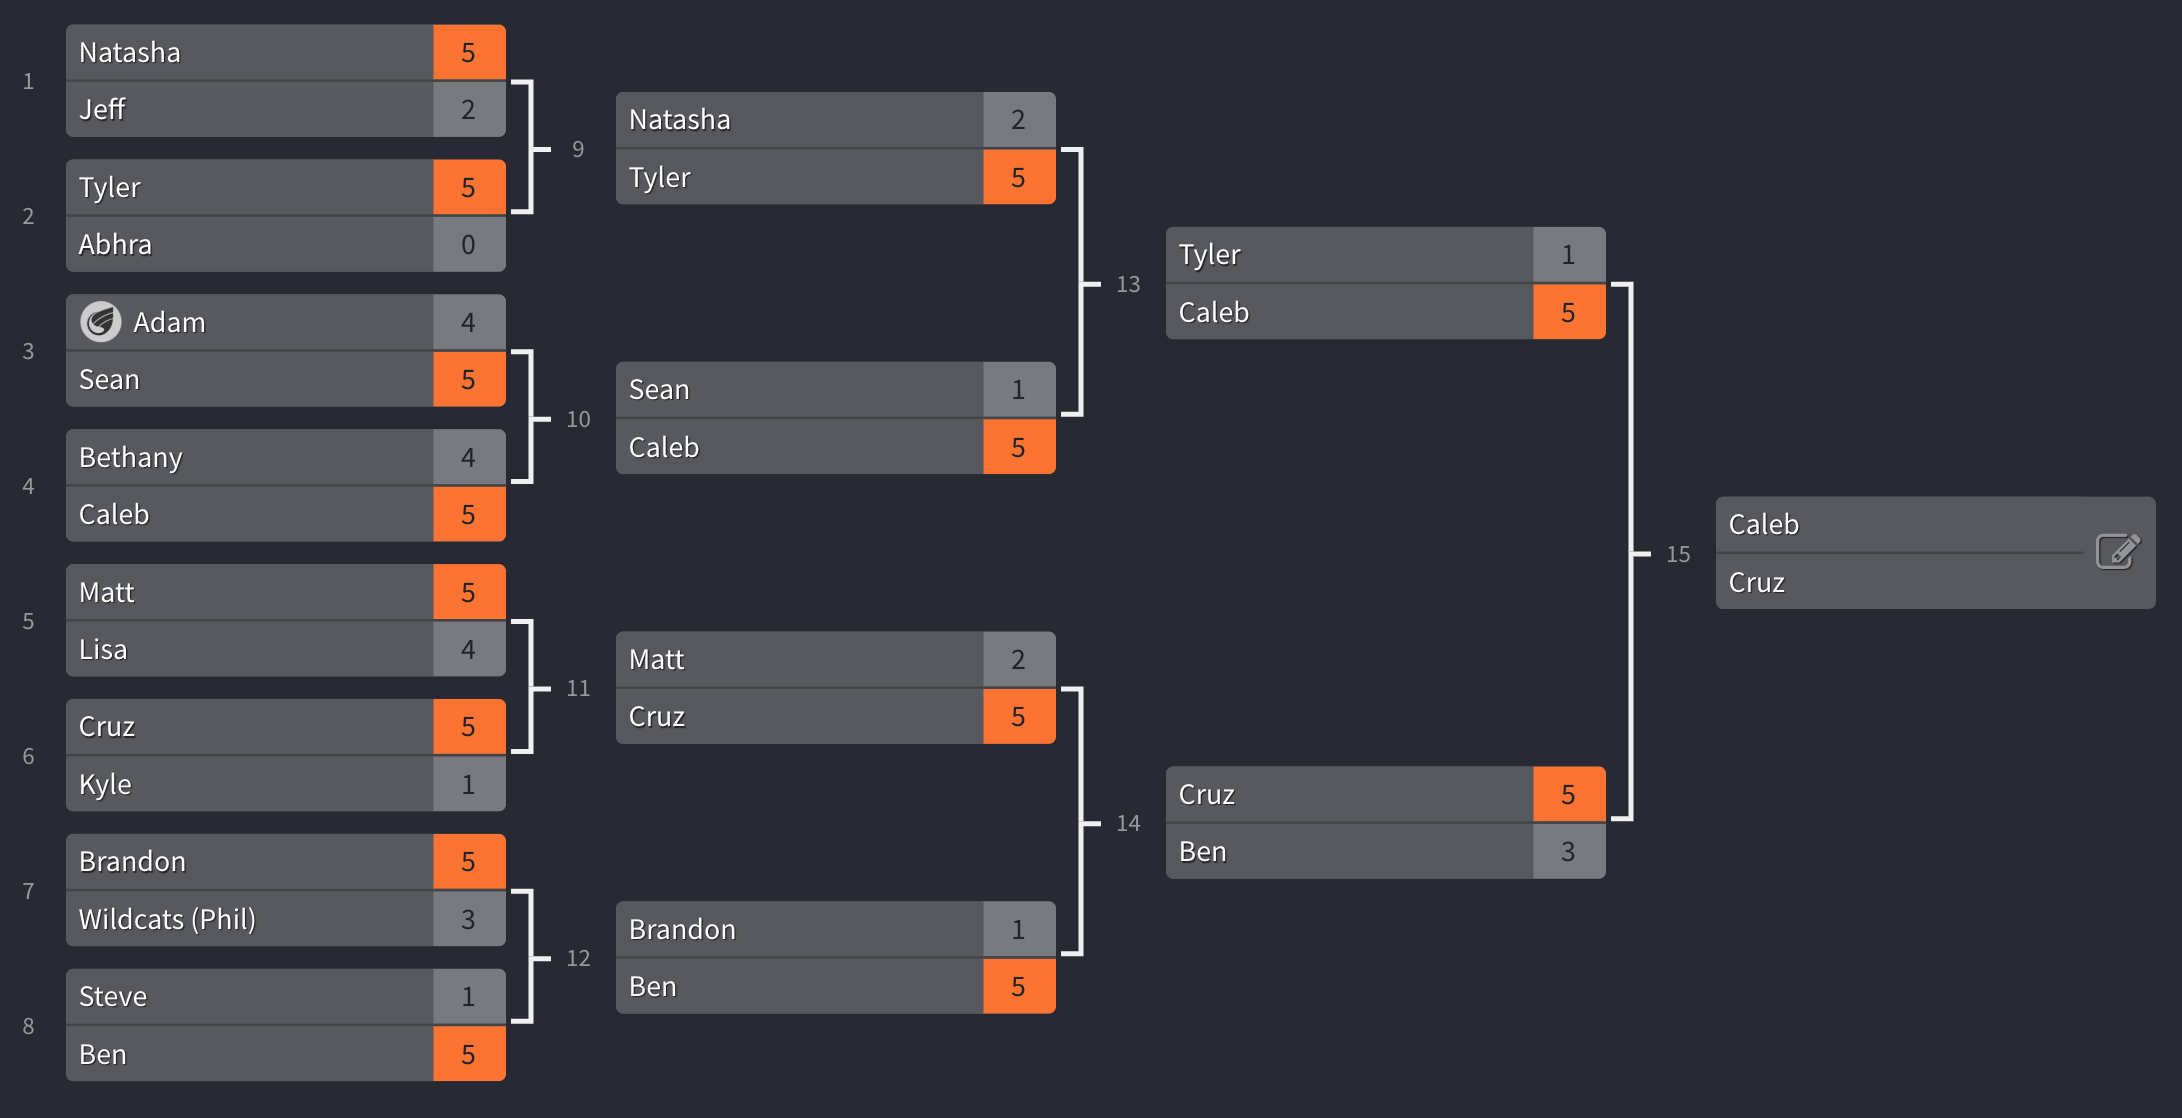
\includegraphics[width=0.9\textwidth]{fig/singles-bracket_6.png}
                \caption{Tournament bracket.}
        \end{subfigure}
        \begin{subfigure}[hb]{0.4\textwidth}
                \footnotesize
                \centering
                \begin{tabular}{lccc}
                        Player	&	$S$	&	$K$	&	$H$	\\
                        \midrule							
                        Abhra	&	-	&	-	&	-	\\
                        Adam	&	$+0.63$	&	-	&	$+0.32$	\\
                        Ben	&	$+0.58$	&	-	&	$+0.29$	\\
                        Bethany	&	$+0.61$	&	-	&	$+0.31$	\\
                        Brandon	&	$+0.47$	&	-	&	$+0.24$	\\
                        Caleb	&	-	&	$-0.55$	&	$-0.28$	\\
                        Cruz	&	$+0.40$	&	-	&	$+0.20$	\\
                        Jeff	&	$+0.65$	&	-	&	$+0.33$	\\
                        Kyle	&	$+0.41$	&	-	&	$+0.20$	\\
                        Lisa	&	$+0.56$	&	-	&	$+0.28$	\\
                        Matt	&	$+1.16$	&	-	&	$+0.58$	\\
                        Natasha	&	$+1.20$	&	-	&	$+0.60$	\\
                        Phil	&	$+0.35$	&	-	&	$+0.18$	\\
                        Sean	&	$+1.22$	&	-	&	$+0.61$	\\
                        Steve	&	$+0.69$	&	-	&	$+0.34$	\\
                        Tyler	&	$-0.41$	&	$+0.80$	&	$+0.20$	\\
                \end{tabular}
                \caption{The HKL sees many changes after this match.}
        \end{subfigure}
        \caption{The HKL correctly predicts Caleb to win against Tyler despite
                 both players entering the match with equal Power Ratings ($K$)
                 and match difficulty $d=1.00$.}
\end{figure}

\clearpage
\subsection{Predicting a winner}

%%%%%%%%%%%%%%%%%%%%%%%%%%%%%%%%%%%%
% \clearpage \section{CASE STUDY: USING INDIVIDUAL HKL RATINGS TO CONDUCT A
% DOUBLES TOURNAMENT} % Show distribution of team HKL using singles HKL for each
% player % Describe how singles ratings are weighted as doubles matches are
% played

% \subsection{Using individual ratings to form well-balanced teams}
% \subsection{Using a weighted HKL to account for an individual's performance in
% a team environment} 

\end{document}
